% Created 2020-07-27 lun 10:56
% Intended LaTeX compiler: pdflatex
\documentclass[presentation,aspectratio=1610]{beamer}
\usepackage[utf8]{inputenc}
\usepackage[T1]{fontenc}
\usepackage{graphicx}
\usepackage{grffile}
\usepackage{longtable}
\usepackage{wrapfig}
\usepackage{rotating}
\usepackage[normalem]{ulem}
\usepackage{amsmath}
\usepackage{textcomp}
\usepackage{amssymb}
\usepackage{capt-of}
\usepackage{hyperref}
\usepackage{khpreamble, euscript}
\DeclareMathOperator{\atantwo}{atan2}
\newcommand*{\ctrb}{\EuScript{C}}
\newcommand*{\obsv}{\EuScript{O}}
\usetheme{default}
\author{Kjartan Halvorsen}
\date{\today}
\title{Control computarizado - Retroalimentación de estados}
\hypersetup{
 pdfauthor={Kjartan Halvorsen},
 pdftitle={Control computarizado - Retroalimentación de estados},
 pdfkeywords={},
 pdfsubject={},
 pdfcreator={Emacs 26.3 (Org mode 9.3.6)}, 
 pdflang={English}}
\begin{document}

\maketitle

\section{Apollo moon lander}
\label{sec:org2a8664b}
\begin{frame}[label={sec:orgee76354}]{Ejemplo - El módulo lunar de Apollo}
\begin{center}
\includegraphics[width=\linewidth]{fig-apollo}
\end{center}
\end{frame}
\begin{frame}[label={sec:orgaf77d3e}]{Ejemplo - El módulo lunar de Apollo}
\begin{center}
\includegraphics[width=0.8\linewidth]{fig-apollo}
\end{center}
\alert{Actividad} ¿Que sensores relevantes se puede usar para el control?
\end{frame}


\begin{frame}[label={sec:orgf07bcc9}]{Ejemplo - El módulo lunar de Apollo}
\begin{center}
\includegraphics[width=0.7\linewidth]{../../figures/mit_LM_autopilot.png}
\end{center}
{\footnotesize ``Dynamics and control challenges during the Apollo project'' MIT OCW}
\end{frame}

\begin{frame}[label={sec:orgf3e0637}]{Ejemplo - El módulo lunar de Apollo}
\begin{center}
\includegraphics[width=0.7\linewidth]{fig-apollo}
\end{center}

Variables del estado: \(x = \begin{bmatrix} x_1 & x_2 & x_3 \end{bmatrix}^T = \begin{bmatrix} \dot{\theta} & \theta & \dot{z} \end{bmatrix}^T\). Con dinamica
\[ \begin{cases} \dot{x}_1 =  \ddot{\theta} = k_1 u\\ \dot{x}_2 = \dot{\theta} = x_1\\ \dot{x}_3 = \ddot{z} = k_2\theta = k_2x_2 \end{cases} \]
\end{frame}

\begin{frame}[label={sec:org7d2985d}]{Ejemplo - El módulo lunar de Apollo}
Variables del estado: \(x = \begin{bmatrix} x_1 & x_2 & x_3 \end{bmatrix}^T = \begin{bmatrix} \dot{\theta} & \theta & \dot{z} \end{bmatrix}^T\). Con dinamica
\[ \begin{cases} \dot{x}_1 =  \ddot{\theta} = k_1 u\\ \dot{x}_2 = \dot{\theta} = x_1\\ \dot{x}_3 = \ddot{z} = k_2\theta = k_2x_2 \end{cases} \]

\[ \dot{x} = \begin{bmatrix} \dot{x}_1\\\dot{x}_2\\\dot{x}_3\end{bmatrix} = \underbrace{\begin{bmatrix} \textcolor{red!60!black}{0} & \textcolor{red!60!black}{0} &\textcolor{red!60!black}{0} \\\textcolor{red!60!black}{1} & \textcolor{red!60!black}{0}& \textcolor{red!60!black}{0}\\ \textcolor{red!60!black}{0}& \textcolor{red!60!black}{k_2} &\textcolor{red!60!black}{0} \end{bmatrix}}_{A} \begin{bmatrix} x_1\\x_2\\x_3\end{bmatrix} + \underbrace{\begin{bmatrix} \textcolor{red!60!black}{k_1} \\ \textcolor{red!60!black}{0} \\\textcolor{red!60!black}{0}  \end{bmatrix}}_{B} u \]
\end{frame}


\section{Matlab demo}
\label{sec:orgbce559a}
\begin{frame}[label={sec:orgb03c156}]{Matlab / Simulink}
\end{frame}

\section{Discretización}
\label{sec:org42dd400}

\begin{frame}[label={sec:org9977e67}]{Discretización}
\end{frame}
\begin{frame}[label={sec:orgc00def8}]{Discretización}
Solución general de un sistema lineal en espacio de estado 
\begin{align*}
x(t_k+\tau)& = \mathrm{e}^{A(\tau)} x(t_k) + \int_{0}^\tau \mathrm{e}^{As} B u\big((t_k+\tau)-s) ds
\end{align*}

\begin{center}
  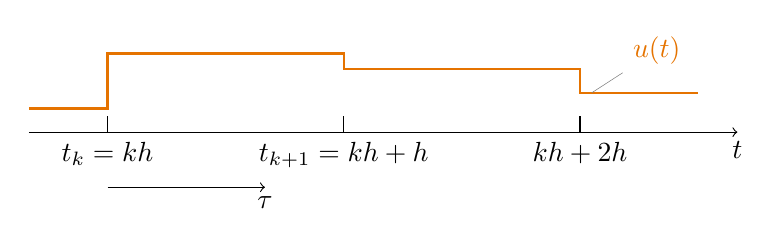
\begin{tikzpicture}
    \draw[->] (-3,0) -- (6,0) node[below] {$t$};
    \draw (-2, 0.2) -- ( -2, 0) node[below] {$t_k=kh$};
    \draw (1, 0.2) -- ( 1, 0) node[below] {$t_{k+1}=kh+h$};
    \draw (4, 0.2) -- ( 4, 0) node[below] {$kh+2h$};
    \draw[thick, orange!90!black] (-3,0.3) -- (-2, 0.3) -- (-2,1) -- (1, 1) -- (1,0.8) -- (4, 0.8) --(4, 0.5) --(5.5, 0.5) node[pos=0.1, coordinate, pin=30:{$u(t)$}] {} ; 
    \draw[->] (-2, -0.7) -- (0, -0.7) node[below] {$\tau$};
  \end{tikzpicture}
\end{center}

 \begin{align*}
  x(kh+h) &= \mathrm{e}^{Ah} x(kh) + \int_{0}^{h} \mathrm{e}^{As} B u(kh+h-s) ds\\
   &= \underbrace{\mathrm{e}^{Ah}}_{\Phi(h)} x(kh) + \underbrace{\left(\int_{0}^h \mathrm{e}^{As} B ds \right)}_{\Gamma(h)} u(kh)
\end{align*}
\end{frame}

\begin{frame}[label={sec:orgd443f9e}]{Discretización - La exponencial de una matriz}
Matriz \(A\) cuadrada. Variable \(t\) escalar.
\[ \mathrm{e}^{At} = 1 + At + \frac{t^2}{2!}A^2 + \frac{t^3}{3!} A^3 + \cdots\]
Transformada de Laplace:
\[ \laplace{\mathrm{e}^{At}} = (sI - A)^{-1}\]
\end{frame}



\begin{frame}[label={sec:orgdb624c7}]{Discretización - Apollo LM}
 \begin{align*}
  x(kh+h) &= \mathrm{e}^{Ah} x(kh) + \int_{0}^{h} \mathrm{e}^{As} B u(kh+h-s) ds\\
   &= \underbrace{\mathrm{e}^{Ah}}_{\Phi(h)} x(kh) + \underbrace{\left(\int_{0}^h \mathrm{e}^{As} B ds \right)}_{\Gamma(h)} u(kh)
\end{align*}
\[ A = \begin{bmatrix} 0 & 0 & 0\\1 & 0 & 0\\0 & k_2 & 0\end{bmatrix}, \quad A^2 = \begin{bmatrix} 0 & 0 & 0\\1 & 0 & 0\\0 & k_2 & 0\end{bmatrix}\begin{bmatrix} 0 & 0 & 0\\1 & 0 & 0\\0 & k_2 & 0\end{bmatrix}= \begin{bmatrix} 0 & 0 & 0\\0 & 0 & 0\\k_2 & 0  & 0\end{bmatrix}, \quad A^3 = 0\]
Entonces,
\begin{align*}
 \Phi(h) &= \mathrm{e}^{Ah} = 1 + Ah + A^2 h^2/2  + \cdots \\
 &= &
 \end{align*}
\end{frame}

\begin{frame}[label={sec:org0ef5b24}]{Discretización - Apollo LM - Solución}
 \begin{align*}
  x(kh+h) &= \mathrm{e}^{Ah} x(kh) + \int_{0}^{h} \mathrm{e}^{As} B u(kh+h-s) ds\\
   &= \underbrace{\mathrm{e}^{Ah}}_{\Phi(h)} x(kh) + \underbrace{\left(\int_{0}^h \mathrm{e}^{As} B ds \right)}_{\Gamma(h)} u(kh)
\end{align*}
\[ A = \begin{bmatrix} 0 & 0 & 0\\1 & 0 & 0\\0 & k_2 & 0\end{bmatrix}, \quad A^2 = \begin{bmatrix} 0 & 0 & 0\\1 & 0 & 0\\0 & k_2 & 0\end{bmatrix}\begin{bmatrix} 0 & 0 & 0\\1 & 0 & 0\\0 & k_2 & 0\end{bmatrix}= \begin{bmatrix} 0 & 0 & 0\\0 & 0 & 0\\k_2 & 0  & 0\end{bmatrix}, \quad A^3 = 0\]
Entonces,
\begin{align*}
 \Phi(h) &= \mathrm{e}^{Ah} = 1 + Ah + A^2 h^2/2  + \cdots \\
 &= \begin{bmatrix} 1 & 0 & 0\\0 & 1 & 0\\0 & 0 & 1\end{bmatrix} + \begin{bmatrix} 0 & 0 & 0\\1 & 0 & 0\\0 & k_2 & 0\end{bmatrix}h + \begin{bmatrix} 0 & 0 & 0\\0 & 0 & 0\\k_2 & 0 & 0\end{bmatrix}\frac{h^ 2}{2}= \begin{bmatrix} 1 & 0 & 0\\h & 1 & 0\\\frac{h^2k_2}{2} & hk_2 & 1\end{bmatrix}
 \end{align*}
\end{frame}

\begin{frame}[label={sec:orga953f08}]{Discretización - Apollo LM}
 \begin{align*}
  x(kh+h) &= \mathrm{e}^{Ah} x(kh) + \int_{0}^{h} \mathrm{e}^{As} B u(kh+h-s) ds\\
   &= \underbrace{\mathrm{e}^{Ah}}_{\Phi(h)} x(kh) + \underbrace{\left(\int_{0}^h \mathrm{e}^{As} B ds \right)}_{\Gamma(h)} u(kh)
\end{align*}
\[\mathrm{e}^{As}B &=  \begin{bmatrix} 1 & 0 & 0\\h & 1 & 0\\\frac{s^2k_2}{2} & sk_2 & 1\end{bmatrix} \begin{bmatrix} k_1\\0\\0 \end{bmatrix} = k_1 \begin{bmatrix} 1\\s\\\frac{k_2s^2}{2} \end{bmatrix}
  \]
\begin{align*}
\Gamma (h) &= \int_0^h \mathrm{e}^{As}B ds =  
\end{align*}
\end{frame}

\begin{frame}[label={sec:org1c38f3d}]{Discretización - Apollo LM - Solución}
 \begin{align*}
  x(kh+h) &= \mathrm{e}^{Ah} x(kh) + \int_{0}^{h} \mathrm{e}^{As} B u(kh+h-s) ds\\
   &= \underbrace{\mathrm{e}^{Ah}}_{\Phi(h)} x(kh) + \underbrace{\left(\int_{0}^h \mathrm{e}^{As} B ds \right)}_{\Gamma(h)} u(kh)\\
   &= \begin{bmatrix} 1 & 0 & 0\\h & 1 & 0\\\frac{h^2k_2}{2} & hk_2 & 1\end{bmatrix} x(kh) + k_1 \begin{bmatrix} h\\ \frac{h^2}{2} \\ \frac{k_2 h^3}{6} \end{bmatrix} u(kh)
\end{align*}
\end{frame}





\section{Estabilidad}
\label{sec:org9f8129d}
\begin{frame}[label={sec:org7a3325f}]{Estabilidad}
\end{frame}
\begin{frame}[label={sec:org3617e74}]{Eigenvalores y eigenvectores}
\alert{Definición} Eigenvalores \(\lambda  \in \mathbb{R}\) y eigenvectores \(v \in \mathbb{R}^n\) de una matriz \(\Phi \in \mathbb{R}^{n\times{}n}\) son pares \((\lambda, v \neq 0 )\) que satisfican
\[ \Phi v = \lambda v \]
\end{frame}

\begin{frame}[label={sec:org5e457e0}]{Estabilidad}
El sistema
\begin{equation*}
x(k+1)=\Phi x(k), \ \ x(0)=x_0
\end{equation*}
es \alert{estable} si  \(\underset{t\to\infty}{\lim}x(kh)=0, \quad \forall\;  x_0\in\Bbb{R}^n\).

Un requisito necessario y suficiente para estabilidad, es que \alert{todos los eigenvalores (valores característicos) de \(\Phi\) están en el interior del círculo unitario.}

Los \alert{eigenvalores} de \(\Phi\) son los \alert{polos} del sistema.
\end{frame}

\section{State feedback}
\label{sec:org6dbb575}
\begin{frame}[label={sec:org703c613}]{Control por retroalimentación de estados}
\end{frame}
\begin{frame}[label={sec:org6d754f6}]{Retroalimentación de estados}
Dado
 \begin{equation}
 \begin{split}
  x(k+1) &= \Phi x(k) + \Gamma u(k)\\
  y(k) &= C x(k)
 \end{split}
 \label{eq:ssmodel}
\end{equation}
y medidas (o valores estimados) del vector de estado \(x(k)\). 

\alert{Reltroalimentación lineal de estados} es la ley de control
\begin{equation*}
\begin{split}
 u(k) &= f\big((x(k), u_c(k)\big) = -l_1x_1(k) - l_2x_2(k) - \cdots - l_n x_n(k) + l_0u_c(k)\\
      &= -Lx(k) + l_0u_c(k), 
\end{split}
\end{equation*}
dónde \[ L = \bbm l_1 & l_2 & \cdots & l_n \ebm. \]
Sustitoyende la ley de control en el modelo en espacio de estado \eqref{eq:ssmodel} da 
 \begin{equation}
 \begin{split}
  x(k+1) &= \left(\Phi -\Gamma L \right) x(k) + m\Gamma u_c(k)\\
  y(k) &= C x(k)
 \end{split}
 \label{eq:closedloop}
\end{equation}
\end{frame}

\begin{frame}[label={sec:org14cc338}]{Asignación de polos por retroalimentación de estados}
Dado ubicación deseada de los polos del lazo cerrado \(p_1, p_2, \ldots, p_n\), correspondiente al polinomio característico deseado
\begin{equation}
a_c(z) = (z-p_1)(z-p_2)\cdots(z-p_n) = z^n + \alpha_1 z^{n-1} + \cdots \alpha_n.
\label{eq:desiredpoles}
\end{equation}

Retroalimentación de estados nos da el sistema 
 \begin{equation}
 \begin{split}
  x(k+1) &= \left(\Phi -\Gamma L \right) x(k) + l_0\Gamma u_c(k)\\
  y(k) &= C x(k)
 \end{split}
 \label{eq:closedloop}
\end{equation}
con polinomio característico
\begin{equation}
\det\left(zI - (\Phi - \Gamma L)\right) = z^n + \beta_1(l_1,\ldots,l_n) z^{n-1} + \cdots \beta_n(l_1, \ldots, l_n).
\label{eq:poles}
\end{equation}

Equipara los coeficientes de \eqref{eq:desiredpoles} con los de \eqref{eq:poles} para obtener sistema de ecuaciones
\begin{equation*}
\begin{split}
\beta_1(l_1, \ldots, l_n) &= \alpha_1\\
\beta_2(l_1, \ldots, l_n) &= \alpha_2\\
&\vdots\\
\beta_n(l_1, \ldots, l_n) &= \alpha_n
\end{split}
\label{eq:coeffs}
\end{equation*}
\end{frame}

\begin{frame}[label={sec:org32b68f3}]{Asignación de polos por retroalimentación de estados}
El sistema de ecuaciones
\begin{equation*}
\begin{split}
\beta_1(l_1, \ldots, l_n) &= \alpha_1\\
\beta_2(l_1, \ldots, l_n) &= \alpha_2\\
&\vdots\\
\beta_n(l_1, \ldots, l_n) &= \alpha_n
\end{split}
\label{eq:coeffs}
\end{equation*}
siempre es lineal en los parámetros del controlador, cuál nos da
\begin{equation*}
M L\transp = \alpha,
\end{equation*}
dónde \(\alpha\transp = \bbm \alpha_1 & \alpha_2 & \cdots & \alpha_n \ebm.\)
\end{frame}

\begin{frame}[label={sec:org6129c37}]{Asignación de polos y controlabilidad}
Se puede verificar que la matriz de controlabilidad 
\[W_c = \bbm \Gamma & \Phi\Gamma & \cdots & \Phi^{n-1}\Gamma\ebm\]
es un factór de la matriz \(M\)
\[ M = \bar{M} W_c. \] Entonces, en general las ecuaciones
\begin{equation}
\bar{M}W_c L\transp = \alpha \qquad \Rightarrow \qquad L\transp = W_c^{-1}\bar{M}^{-1}\alpha
\label{eq:poleplace}
\end{equation}
solo tienen una solución si \(W_c\) es invertible, es decir cuando el sistema es \emph{controlable}.

 Nota que las ecuaciones \eqref{eq:poleplace} pueden tener soluciónes (numero infinito) cuando el sistema no es controlable, si  \alert{\(\alpha\) está en el espacio de columnas de \(M\)}. Es decir, se puede escribir 
\[ \alpha = b_1 M_{:,1} + b_2M_{:,2} + \cdots + b_M_{:,m}, \; m < n \]
\end{frame}

\begin{frame}[label={sec:orgc7adc48},fragile]{Asignación de polos por retroalimentación de estados}
 Dado ubicación deseada de los polos del lazo cerrado \(p_1, p_2, \ldots, p_n\), correspondiente al polinomio característico deseado
\begin{equation}
a_c(z) = (z-p_1)(z-p_2)\cdots(z-p_n) = z^n + \alpha_1 z^{n-1} + \cdots \alpha_n.
\end{equation}
y sistema de espacio de estado en lazo cerrado
 \begin{equation}
 \begin{split}
  x(k+1) &= \left(\Phi -\Gamma L \right) x(k) + l_0\Gamma u_c(k)\\
  y(k) &= C x(k)
 \end{split}
\end{equation}

Matlab (\emph{control systems toolbox}) tiene dos métodos para calcular las ganancias \(L\)

\begin{enumerate}
\item \alert{Método de Ackerman} 
\begin{verbatim}
L = acker(Phi, Gamma, pd)
\end{verbatim}
\item \alert{Método numericamente estable} 
\begin{verbatim}
L = place(Phi, Gamma, pd)
\end{verbatim}
\end{enumerate}
\end{frame}

\begin{frame}[label={sec:org6e2cc41}]{La ganancia \(l_0\) de la referencia}
El sistema de espacio de estado en lazo cerrado
\begin{equation*}
\begin{split}
 x(k+1) &= \underbrace{\left(\Phi -\Gamma L \right)}_{\Phi_c} x(k) + l_0\Gamma u_c(k)\\
 y(k) &= C x(k)
\end{split}
\end{equation*}
tiene la solución en estado estacionario (\(x(k+1)=x(k)\)) con referencia constante \(u_c(k) = u_{c,f}\)
\[ y_f = l_0 C(I - \Phi_c)^{-1}\Gamma u_{c,f}.\]
Queremos \(y_f =  u_{c,f}\),
\[ \Rightarrow \qquad l_0 = \frac{1}{C(I-\Phi_c)^{-1}\Gamma}\]
\end{frame}

\begin{frame}[label={sec:orgb814396}]{Matlab}
\end{frame}
\begin{frame}[label={sec:orge2ee402}]{Actividad}
En grupos: 
\begin{enumerate}
\item Visualiza la atitúd (angulo \(\theta\) en grados) del módulo lunar durante la simulación. Cuál es el angulo máximo?
\item Determina las ganancias \(L = \bbm l_1 & l_2 & l_3 \ebm\) para control \emph{dead-beat}. Es decir con todos los polos del sistema en lazo cerrado en el origen.
\item Simula el sistema en lazo cerrado con control dead-beat. Cuál es el angulo máximo del módulo lunar?
\item Cambia el periodo de muestreo de \(h=1\)s a \(h=0.5\)s. Cuál es el angulo máximo ahora, usando control  dead-beat.
\end{enumerate}
\end{frame}
\end{document}